% Politecnico di Milano (PoliMi) - School of Industrial and Information Engineering
%
% Copyright 2021 Politecnico di Milano, Italy. NC-BY

\documentclass{Configuration_Files/Template}

%------------------------------------------------------------------------------
%	REQUIRED PACKAGES AND  CONFIGURATIONS
%------------------------------------------------------------------------------

% CONFIGURATIONS
\usepackage{parskip} % For paragraph layout
\usepackage{setspace} % For using single or double spacing
\usepackage{emptypage} % To insert empty pages
\usepackage{multicol} % To write in multiple columns (executive summary)
\setlength\columnsep{15pt} % Column separation in executive summary
\setlength\parindent{0pt} % Indentation
\raggedbottom  

% PACKAGES FOR TITLES
\usepackage{titlesec}
% \titlespacing{\section}{left spacing}{before spacing}{after spacing}
\titlespacing{\section}{0pt}{3.3ex}{2ex}
\titlespacing{\subsection}{0pt}{3.3ex}{1.65ex}
\titlespacing{\subsubsection}{0pt}{3.3ex}{1ex}
\usepackage{color}

% PACKAGES FOR LANGUAGE AND FONT
\usepackage[english]{babel} % The document is in English  
\usepackage[utf8]{inputenc} % UTF8 encoding
\usepackage[T1]{fontenc} % Font encoding
\usepackage[11pt]{moresize} % Big fonts

% PACKAGES FOR IMAGES
\usepackage{graphicx}
\usepackage{transparent} % Enables transparent images
\usepackage{eso-pic} % For the background picture on the title page
\usepackage{subfig} % Numbered and caption subfigures using \subfloat.
\usepackage{tikz} % A package for high-quality hand-made figures.
\usetikzlibrary{}
\graphicspath{{./Images/}} % Directory of the images
\usepackage{caption} % Coloured captions
\usepackage{amsthm,thmtools,xcolor} % Coloured "Theorem"
\usepackage{float}

% STANDARD MATH PACKAGES
\usepackage{amsmath}
\usepackage{amsthm}
\usepackage{amssymb}
\usepackage{amsfonts}
\usepackage{bm}
\usepackage[overload]{empheq} % For braced-style systems of equations.
\usepackage{fix-cm} % To override original LaTeX restrictions on sizes

% PACKAGES FOR TABLES
\usepackage{tabularx}
\usepackage{longtable} % Tables that can span several pages
\usepackage{colortbl}

% PACKAGES FOR ALGORITHMS (PSEUDO-CODE)
\usepackage{algorithm}
\usepackage{algorithmic}

% PACKAGES FOR REFERENCES & BIBLIOGRAPHY
\usepackage[colorlinks=true,linkcolor=black,anchorcolor=black,citecolor=black,filecolor=black,menucolor=black,runcolor=black,urlcolor=black]{hyperref} % Adds clickable links at references
\usepackage{cleveref}
\usepackage[square, numbers, sort&compress]{natbib} % Square brackets, citing references with numbers, citations sorted by appearance in the text and compressed
\bibliographystyle{abbrvnat} % You may use a different style adapted to your field

% OTHER PACKAGES
\usepackage{pdfpages} % To include a pdf file
\usepackage{afterpage}
\usepackage{lipsum} % DUMMY PACKAGE
\usepackage{fancyhdr} % For the headers
\fancyhf{}

% Input of configuration file. Do not change config.tex file unless you really know what you are doing. 
% Define blue color typical of polimi
\definecolor{bluepoli}{cmyk}{0.4,0.1,0,0.4}

% Custom theorem environments
\declaretheoremstyle[
  headfont=\color{bluepoli}\normalfont\bfseries,
  bodyfont=\color{black}\normalfont\itshape,
]{colored}

% Set-up caption colors
\captionsetup[figure]{labelfont={color=bluepoli}} % Set colour of the captions
\captionsetup[table]{labelfont={color=bluepoli}} % Set colour of the captions
\captionsetup[algorithm]{labelfont={color=bluepoli}} % Set colour of the captions

\theoremstyle{colored}
\newtheorem{theorem}{Theorem}[chapter]
\newtheorem{proposition}{Proposition}[chapter]

% Enhances the features of the standard "table" and "tabular" environments.
\newcommand\T{\rule{0pt}{2.6ex}}
\newcommand\B{\rule[-1.2ex]{0pt}{0pt}}

% Pseudo-code algorithm descriptions.
\newcounter{algsubstate}
\renewcommand{\thealgsubstate}{\alph{algsubstate}}
\newenvironment{algsubstates}
  {\setcounter{algsubstate}{0}%
   \renewcommand{\STATE}{%
     \stepcounter{algsubstate}%
     \Statex {\small\thealgsubstate:}\space}}
  {}

% New font size
\newcommand\numfontsize{\@setfontsize\Huge{200}{60}}

% Title format: chapter
\titleformat{\chapter}[hang]{
\fontsize{50}{20}\selectfont\bfseries\filright}{\textcolor{bluepoli} \thechapter\hsp\hspace{2mm}\textcolor{bluepoli}{|   }\hsp}{0pt}{\huge\bfseries \textcolor{bluepoli}
}

% Title format: section
\titleformat{\section}
{\color{bluepoli}\normalfont\Large\bfseries}
{\color{bluepoli}\thesection.}{1em}{}

% Title format: subsection
\titleformat{\subsection}
{\color{bluepoli}\normalfont\large\bfseries}
{\color{bluepoli}\thesubsection.}{1em}{}

% Title format: subsubsection
\titleformat{\subsubsection}
{\color{bluepoli}\normalfont\large\bfseries}
{\color{bluepoli}\thesubsubsection.}{1em}{}

% Shortening for setting no horizontal-spacing
\newcommand{\hsp}{\hspace{0pt}}

\makeatletter
% Renewcommand: cleardoublepage including the background pic
\renewcommand*\cleardoublepage{%
  \clearpage\if@twoside\ifodd\c@page\else
  \null
  \AddToShipoutPicture*{\BackgroundPic}
  \thispagestyle{empty}%
  \newpage
  \if@twocolumn\hbox{}\newpage\fi\fi\fi}
\makeatother

%For correctly numbering algorithms
\numberwithin{algorithm}{chapter}

%----------------------------------------------------------------------------
%	NEW COMMANDS DEFINED
%----------------------------------------------------------------------------

% EXAMPLES OF NEW COMMANDS
\newcommand{\bea}{\begin{eqnarray}} % Shortcut for equation arrays
\newcommand{\eea}{\end{eqnarray}}
\newcommand{\e}[1]{\times 10^{#1}}  % Powers of 10 notation

%----------------------------------------------------------------------------
%	ADD YOUR PACKAGES (be careful of package interaction)
%----------------------------------------------------------------------------

\usepackage{geometry}
\usepackage{tabularx}
\usepackage{booktabs,xltabular}
\usepackage{hyperref}
\usepackage{listings}

%----------------------------------------------------------------------------
%	ADD YOUR DEFINITIONS AND COMMANDS (be careful of existing commands)
%----------------------------------------------------------------------------

% Set uniform margins
\geometry{
  left=0.8in,
  right=0.8in,
  top=1in,
  bottom=1in,
  includehead,
  includefoot
}

%----------------------------------------------------------------------------
%	BEGIN OF YOUR DOCUMENT
%----------------------------------------------------------------------------

\begin{document}

\fancypagestyle{plain}{%
\fancyhf{} % Clear all header and footer fields
\fancyhead[RO,RE]{\thepage} %RO=right odd, RE=right even
\renewcommand{\headrulewidth}{0pt}
\renewcommand{\footrulewidth}{0pt}}

%----------------------------------------------------------------------------
%	TITLE PAGE
%----------------------------------------------------------------------------

\pagestyle{empty} % No page numbers
\frontmatter % Use roman page numbering style (i, ii, iii, iv...) for the preamble pages

\puttitle{
    title= Numerical Analysis for ML,
    name= {Mattia Piccinato},
    academicyear= {2023-24},
    link= \href{https://github.com/peetceenatoo/movierec}{Click here}

 }

%----------------------------------------------------------------------------
%	PREAMBLE PAGES: ABSTRACT (inglese e italiano), EXECUTIVE SUMMARY
%----------------------------------------------------------------------------
\startpreamble
\setcounter{page}{1} % Set page counter to 1

%----------------------------------------------------------------------------
%	LIST OF CONTENTS/FIGURES/TABLES/SYMBOLS
%----------------------------------------------------------------------------

% TABLE OF CONTENTS
\thispagestyle{empty}
\tableofcontents % Table of contents 
\thispagestyle{empty}
\cleardoublepage

%-------------------------------------------------------------------------
%	MAIN TEXT
%-------------------------------------------------------------------------.

\addtocontents{toc}{\vspace{2em}} % Add a gap in the Contents, for aesthetics
\mainmatter % Begin numeric (1,2,3...) page numbering

% FIRST CHAPTER
% --------------------------------------------------------------------------
\chapter{Scope}

\section{Introduction}

The referenced paper introduces a movie recommendation system called \textbf{MOVREC}. This system employs a \textbf{collaborative filtering approach}, using user-provided information to analyze and recommend movies \textbf{without personalization}.

The recommended movie list is generated using the \textbf{K-means algorithm} to cluster the movies in the dataset. It includes movies belonging to the cluster with the \textbf{highest average rating} and sorts them based on their individual ratings.

The paper addresses the common challenge individuals face since the web appearance: an overload of choices. In response, companies deploy recommendation systems to assist users by \textbf{suggesting a small cluster of movies, rather than the entire dataset}.

\section{Aim}

As the paper did not report any results, the identified scope for this project was to \textbf{implement the recommender system} in order to verify its functionality.


% SECOND CHAPTER
% --------------------------------------------------------------------------
\chapter{MOVREC Main Aspects}

\section{Collaborative Filtering}

Collaborative filtering systems recommend items based on similarity measures between users rather than items, providing serendipitous recommendations as they rely on user similarity rather than item similarity.

In particular, MOVREC implements a straightforward approach that aims to recommend \textbf{items preferred by the majority of users}.

\section{Explicit Rating}

Explicit ratings provided by users serve as a crucial input for predicting their movie choices.

Among the attributes of each movie, namely directors, actors, year, genre, and average rating, the latter represents the average of all ratings given by users. \textbf{The system leverages the average rating} to suggest items that are most likely to be enjoyed.

\section{Data Filtering}

Data filtering refers to the process of selectively extracting or excluding data from a dataset based on specific criteria or conditions. The goal of data filtering is to focus on relevant information or remove unwanted elements, making it easier to analyze or visualize the data.

Users are given the choice to select values for different attributes. Based on these input values, the system computes an array of suitable movies, with \textbf{at least one attribute value} that matches the input value of the user. Then, \textbf{only the top 20 movies} by rating are considered, prioritizing those that received more ratings.

\section{K-Means Algorithm}

In the K-means clustering technique, K initial centroids are chosen and assigned to the cluster with the nearest centroid. The centroid of each cluster is then updated, and the process is repeated until convergence. It aims to minimize the following objective function:

\begin{equation}
    J = \sum_{i=1}^{k} \sum_{j=1}^{n} d(x_j, c_i)^2
\end{equation}

Here, \(n\) is the number of cases, \(k\) is the number of clusters, \(d\) is a distance measure, \(c_i\) is a cluster center, and \(x_j\) is a data point.

The system utilizes the K-Means Algorithm to form \textbf{moderately-sized clusters} of movies. This approach helps with presenting a concise list of recommended movies, \textbf{belonging to the cluster expected to better predict user choices}.

\section{Movies Weights}

To compute the average rating of a cluster, the system assigns different weights to each movie \(m\). The weight \(W_m\) of each movie is computed as the sum of the weights given to the value of their \(f\) attributes.

\begin{equation}
    W_m = \sum_{j=1}^{f} w_j
\end{equation}

For the average rating, this is the table of the possible weights:

\begin{figure}[H]
    \centering
    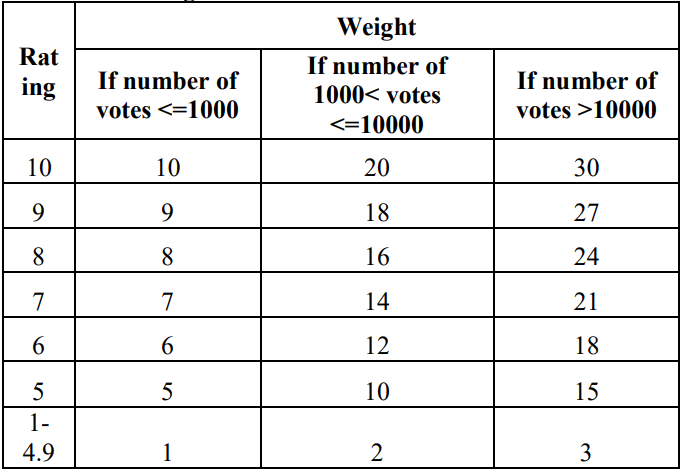
\includegraphics[width=0.4\linewidth]{NAML_latex//Images/RatingWeight.png}
\end{figure}

While the weights for the other attributes' values are defined as the frequency of that value along the entire dataset (for the year, for the actors, for the directors, and for the genre).

\begin{equation}
    w_j = \frac{\text{count of movies with } F_j = f_j}{\text{total number of movies}}
\end{equation}

Overall, the average rating for the cluster is computed, giving \textbf{more importance to movies with a higher rating}, thus choosing clusters with a higher percentage of "good movies," as well as giving priority to those movies with \textbf{common features}.


% THIRD CHAPTER
% --------------------------------------------------------------------------
\chapter{Methodology}

\section{Dataset Cleaning}

\subsection{Selected Dataset}

As mentioned in the paper, the dataset was obtained from \textbf{\href{www.imdb.com}{www.imdb.com}} due to its extensive collection of movies and ratings from a large number of users.

\subsection{Operations on the Dataset}

To create a dataset with information on actors, directors, genre, year, and average rating, \textbf{three different datasets were merged}. Unnecessary columns were \textbf{dropped} from each, and \textbf{rows with null values were removed}.

Note that the column containing the number of ratings was retained to filter the best 20 movies before the clustering process.

\subsection{Weights Pre-processing}

The movie weights were then \textbf{pre-processed} and added as a new column in the dataset.

\subsection{Frameworks and Technologies}

This section outlines the operations performed to obtain the dataset in \(get\_datasets.ipynb\).

\textbf{\href{https://pandas.pydata.org}{Pandas}} dataframes were used to perform these operations efficiently and store the data in the \(dataset.csv\).

\section{Workflow}

\subsection{Filter Function}

The initial implementation involved the \textbf{filter function}.

As stated in the paper, conditions on movie attributes can be specified, and the function returns the \textbf{entire dataset dataframe} if no condition is defined. Otherwise, it returns the \textbf{dataframe containing movies that satisfy at least one} condition.

\subsection{Recommender Function}

Next, the \textbf{recommender function} was implemented.

The first task was to choose an \textbf{appropriate number of clusters}. The default number is assumed to be 4 to return a recommendation cluster containing an average of 5 movies. However, if the filtered list contains fewer than 20 movies, the number of clusters is proportionally resized.\\

\begin{figure}[H]
    \centering
    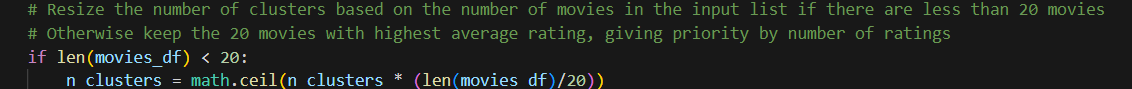
\includegraphics[width=1\linewidth]{NAML_latex//Images/NumOfClusters.png}
    \caption{Resizing the number of clusters.}
\end{figure}

The second task involved \textbf{selecting only the best 20 movies} based on average rating and number of ratings if the filtered list still contains more than 20 movies. After this selection, the column representing the number of ratings for each movie was dropped from the dataframe.\\

\begin{figure}[H]
    \centering
    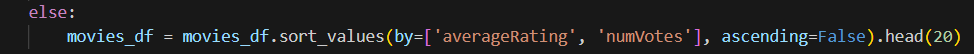
\includegraphics[width=1\linewidth]{NAML_latex//Images/Top20.png}
    \caption{Select the top 20 movies.}
\end{figure}

At this point, the \textbf{K-Means Algorithm} was implemented. Although Euclidean distance is sensitive to categorical data, it was chosen as per the paper's recommendation. To represent categorical data, \textbf{One-Hot encoding} was used for sets of directors, authors, and genres, and the Hamming Distance was chosen to calculate the distance along each "axis".\\

\begin{figure}[H]
    \centering
    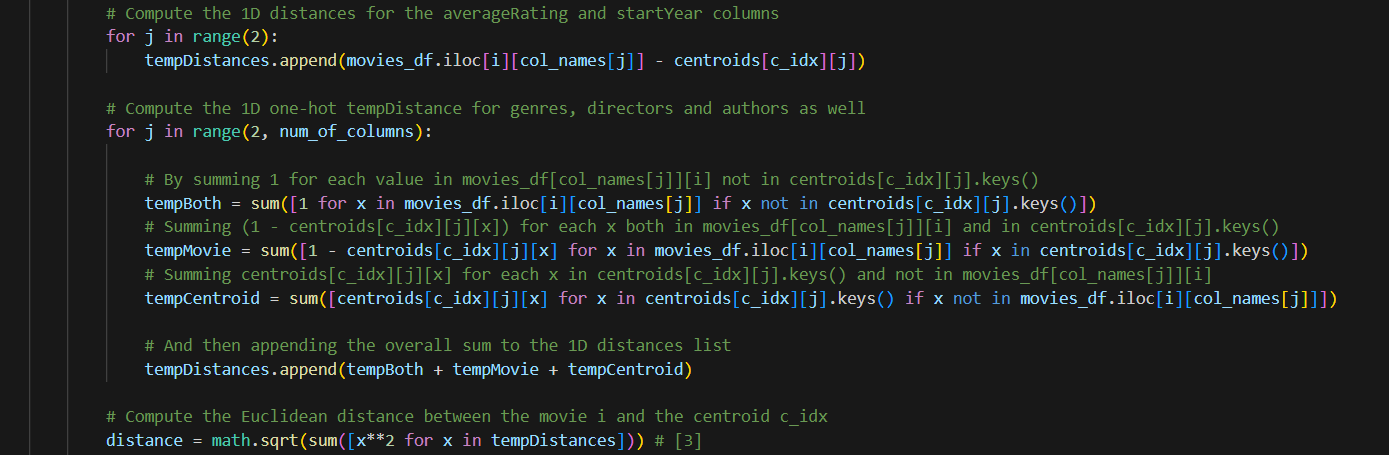
\includegraphics[width=1\linewidth]{NAML_latex//Images/Distance.png}
    \caption{Euclidean distance.}
\end{figure}

Finally, the \textbf{best cluster} was chosen based on the weighted average rating of the cluster.\\

\begin{figure}[H]
    \centering
    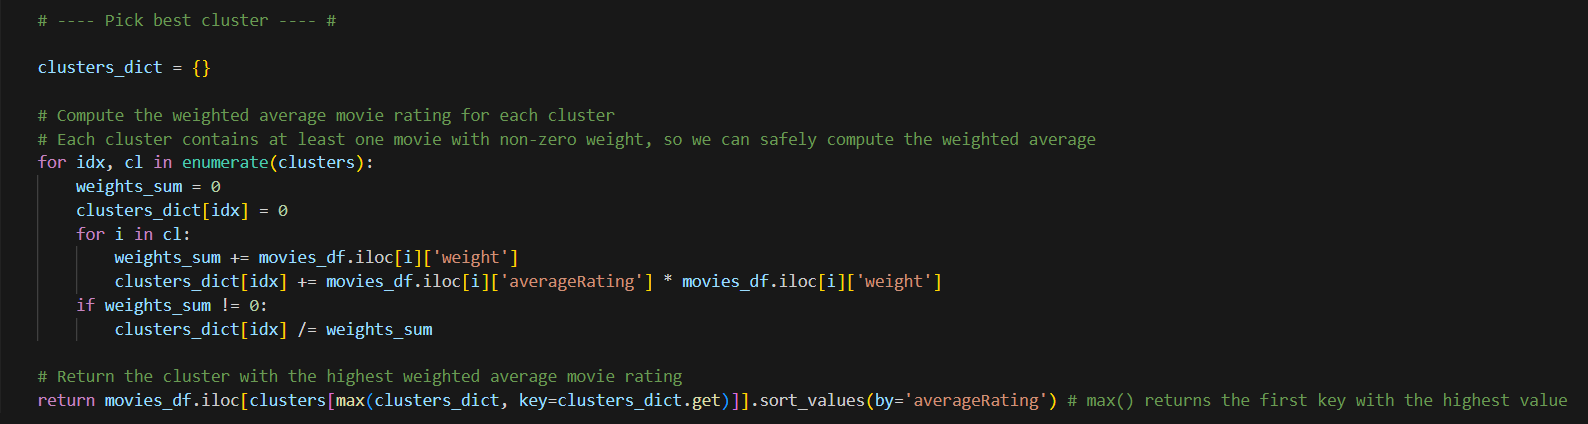
\includegraphics[width=1\linewidth]{NAML_latex//Images/BestCluster.png}
    \caption{Selection of the best cluster.}
    \label{fig:enter-label}
\end{figure}

\subsection{Frameworks and Technologies}

This section illustrates the implementation in \(implementation.ipynb\).

\textbf{\href{https://pandas.pydata.org}{Pandas}} dataframes were used to facilitate these operations.


% FOURTH CHAPTER
% --------------------------------------------------------------------------
\chapter{Results and Conclusions}

As stated in the paper: \textit{"Given the nature of our system, evaluating performance is challenging since there is \textbf{no definitive right or wrong recommendation}; it is purely a matter of opinions."}

Therefore, only a couple of functionality tests were performed. These include verifying that the recommendations are \textbf{deterministic} and exploring the system's response to different filtering choices.

Notably, \textbf{filtering by low values for the rating field is often ineffective in combination with other filter options}.

\end{document}
